\colorlet{outlinecolor}{brightpurple}

\colorlet{headercolor}{outlinecolor}
\colorlet{rowcolor1}{outlinecolor!70}
\colorlet{rowcolor2}{outlinecolor!50}

\definecolor{emphasiscolor}{HTML}{DA70D6}

\begin{tikzpicture}
	\node [mybox, fill=boxcolor, draw=outlinecolor] (box){%
		\begin{minipage}{0.3\textwidth}
			\vspace{0.1cm}
			
			\underline{Introduction}: It's a best practice to create all your changes on \textcolor{emphasiscolor}{feature (or topic) branches}, make sure these changes stable, and then merge into the \inlinebash{main} branch.
			
			\vspace{-2mm}
			\begin{center}
				\textcolor{background}{
					\begin{tabularx}{\textwidth}{>{\columncolor{rowcolor1}}X|>{\columncolor{rowcolor2}}p{3.5cm}}
						\arrayrulecolor{boxcolor} % Table line color
						\rowcolor{headercolor} % Header row color
						\multicolumn{1}{c|}{\centering \textbf{Git Command}} & \multicolumn{1}{c}{\centering \textbf{Description}} \\ % Center the header text
						\hline % Add a horizontal line below the header row
						\rowcolor{rowcolor1} % New Row
						\tablebash{git branch} & Lists all current \textbf{local} branches \\
						\rowcolor{rowcolor2} 
						\tablebash{git branch --all} & Lists all current local and remote branches \\
						\rowcolor{rowcolor1} 
						\tablebash{git branch -m old\_branch\_name new\_branch\_name} & Rename your Git branch \\
						\rowcolor{rowcolor2} 
						\tablebash{git branch --delete branch\_name} & Deletes a \textbf{local} branch\\
					\end{tabularx}
				}
			\end{center}
			\vspace{-1mm}
			
			\underline{Merging}: Insert the changes from one branch into another \textcolor{emphasiscolor}{as a new commit}. Main types of merges are:
			\begin{itemize}
				\item A \textcolor{emphasiscolor}{fast forward merge} happens when one branch is ahead of another. i.e.,
			\end{itemize}
			% Start figure
			\hfill
			\begin{minipage}{0.45\textwidth} 
				\centering
				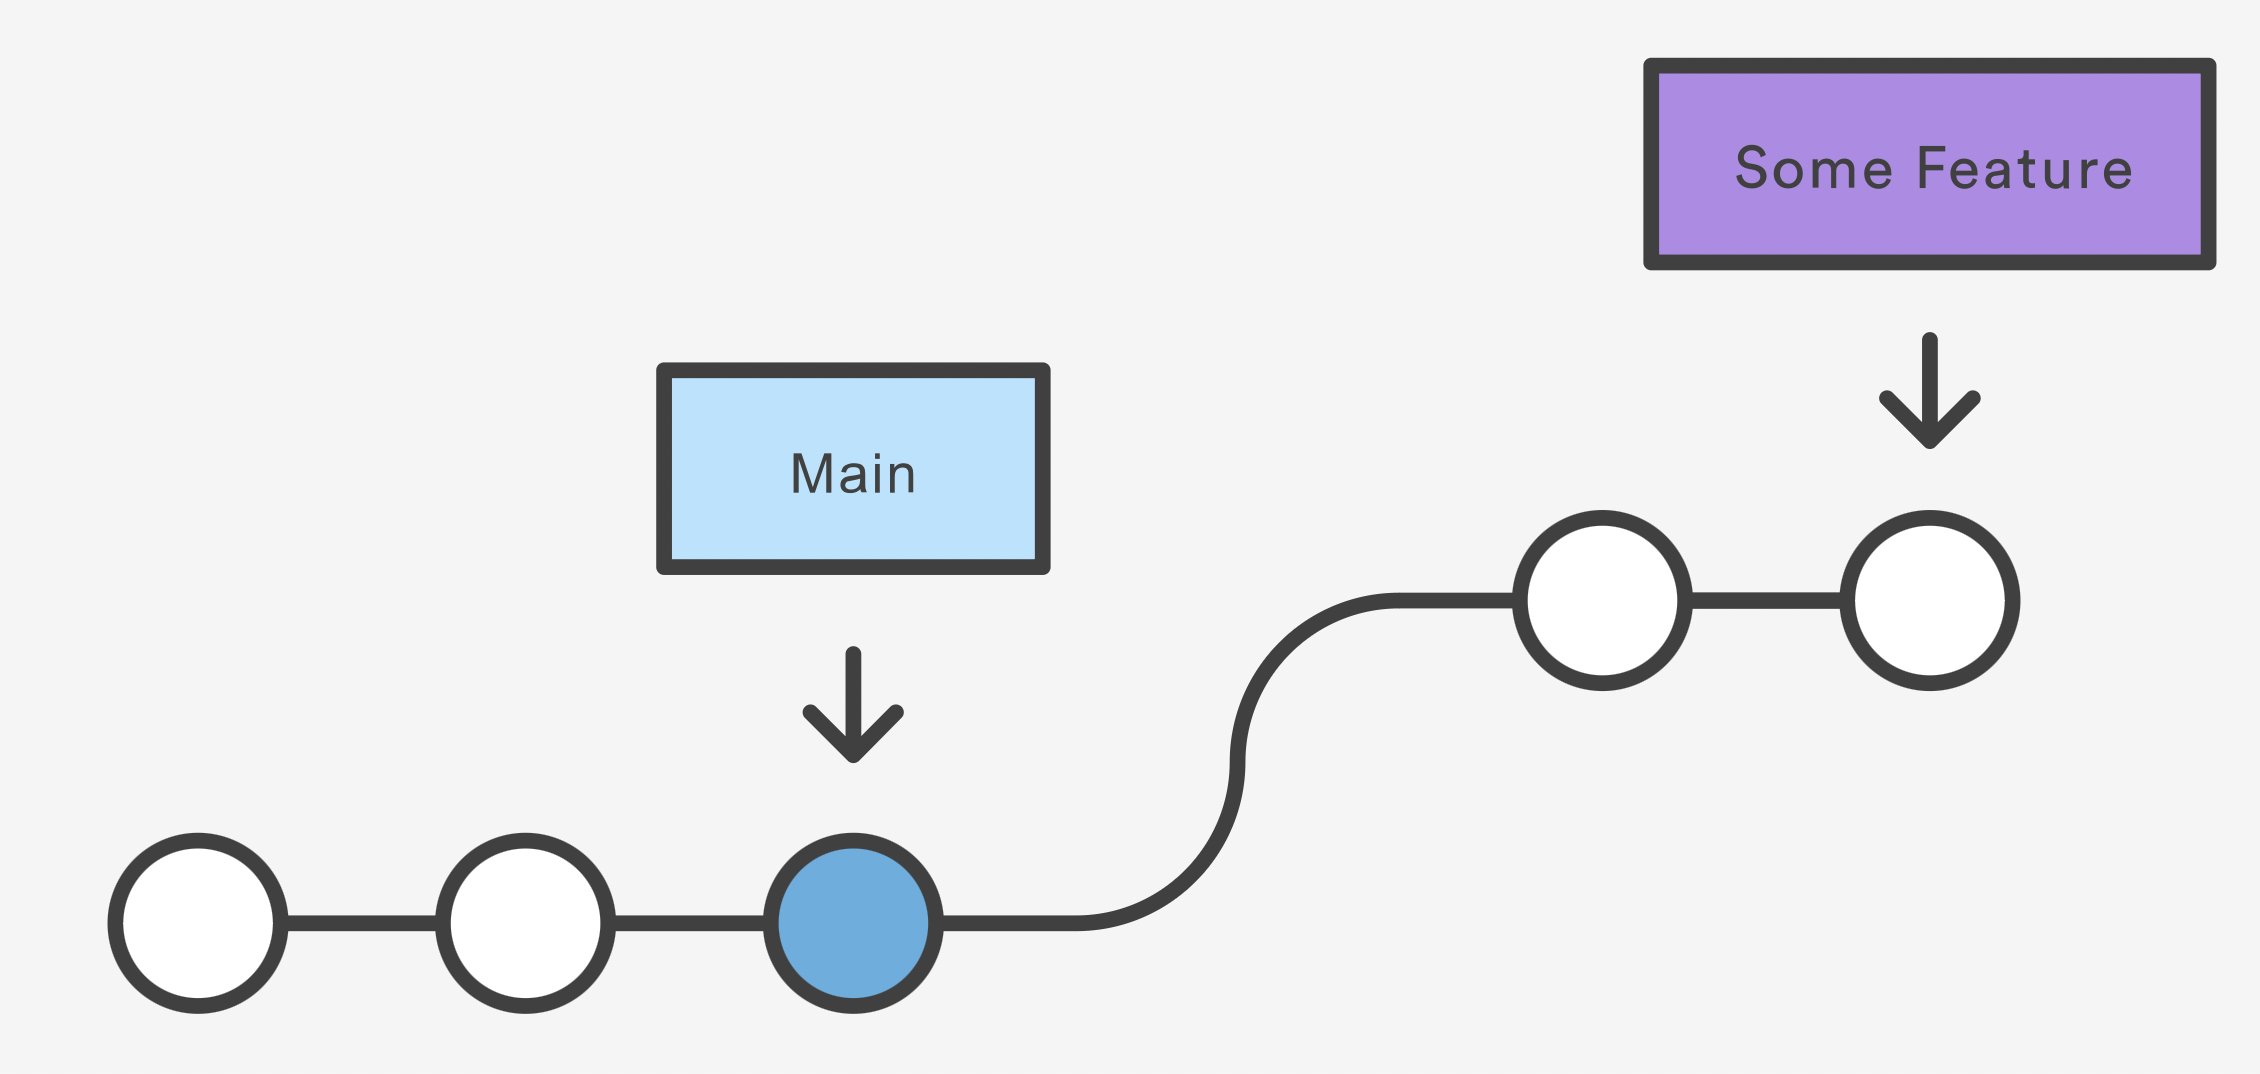
\includegraphics[width=\textwidth]{images/fast_forward_merge_before.png}
				\captionsetup{justification=centering}
				\captionof{figure}{Before fast-forward merge. \href{https://www.atlassian.com/git/tutorials/using-branches/git-merge}{\faLink{} Source}}
			\end{minipage}%
			\hfill
			\begin{minipage}{0.4\textwidth}
				\centering
				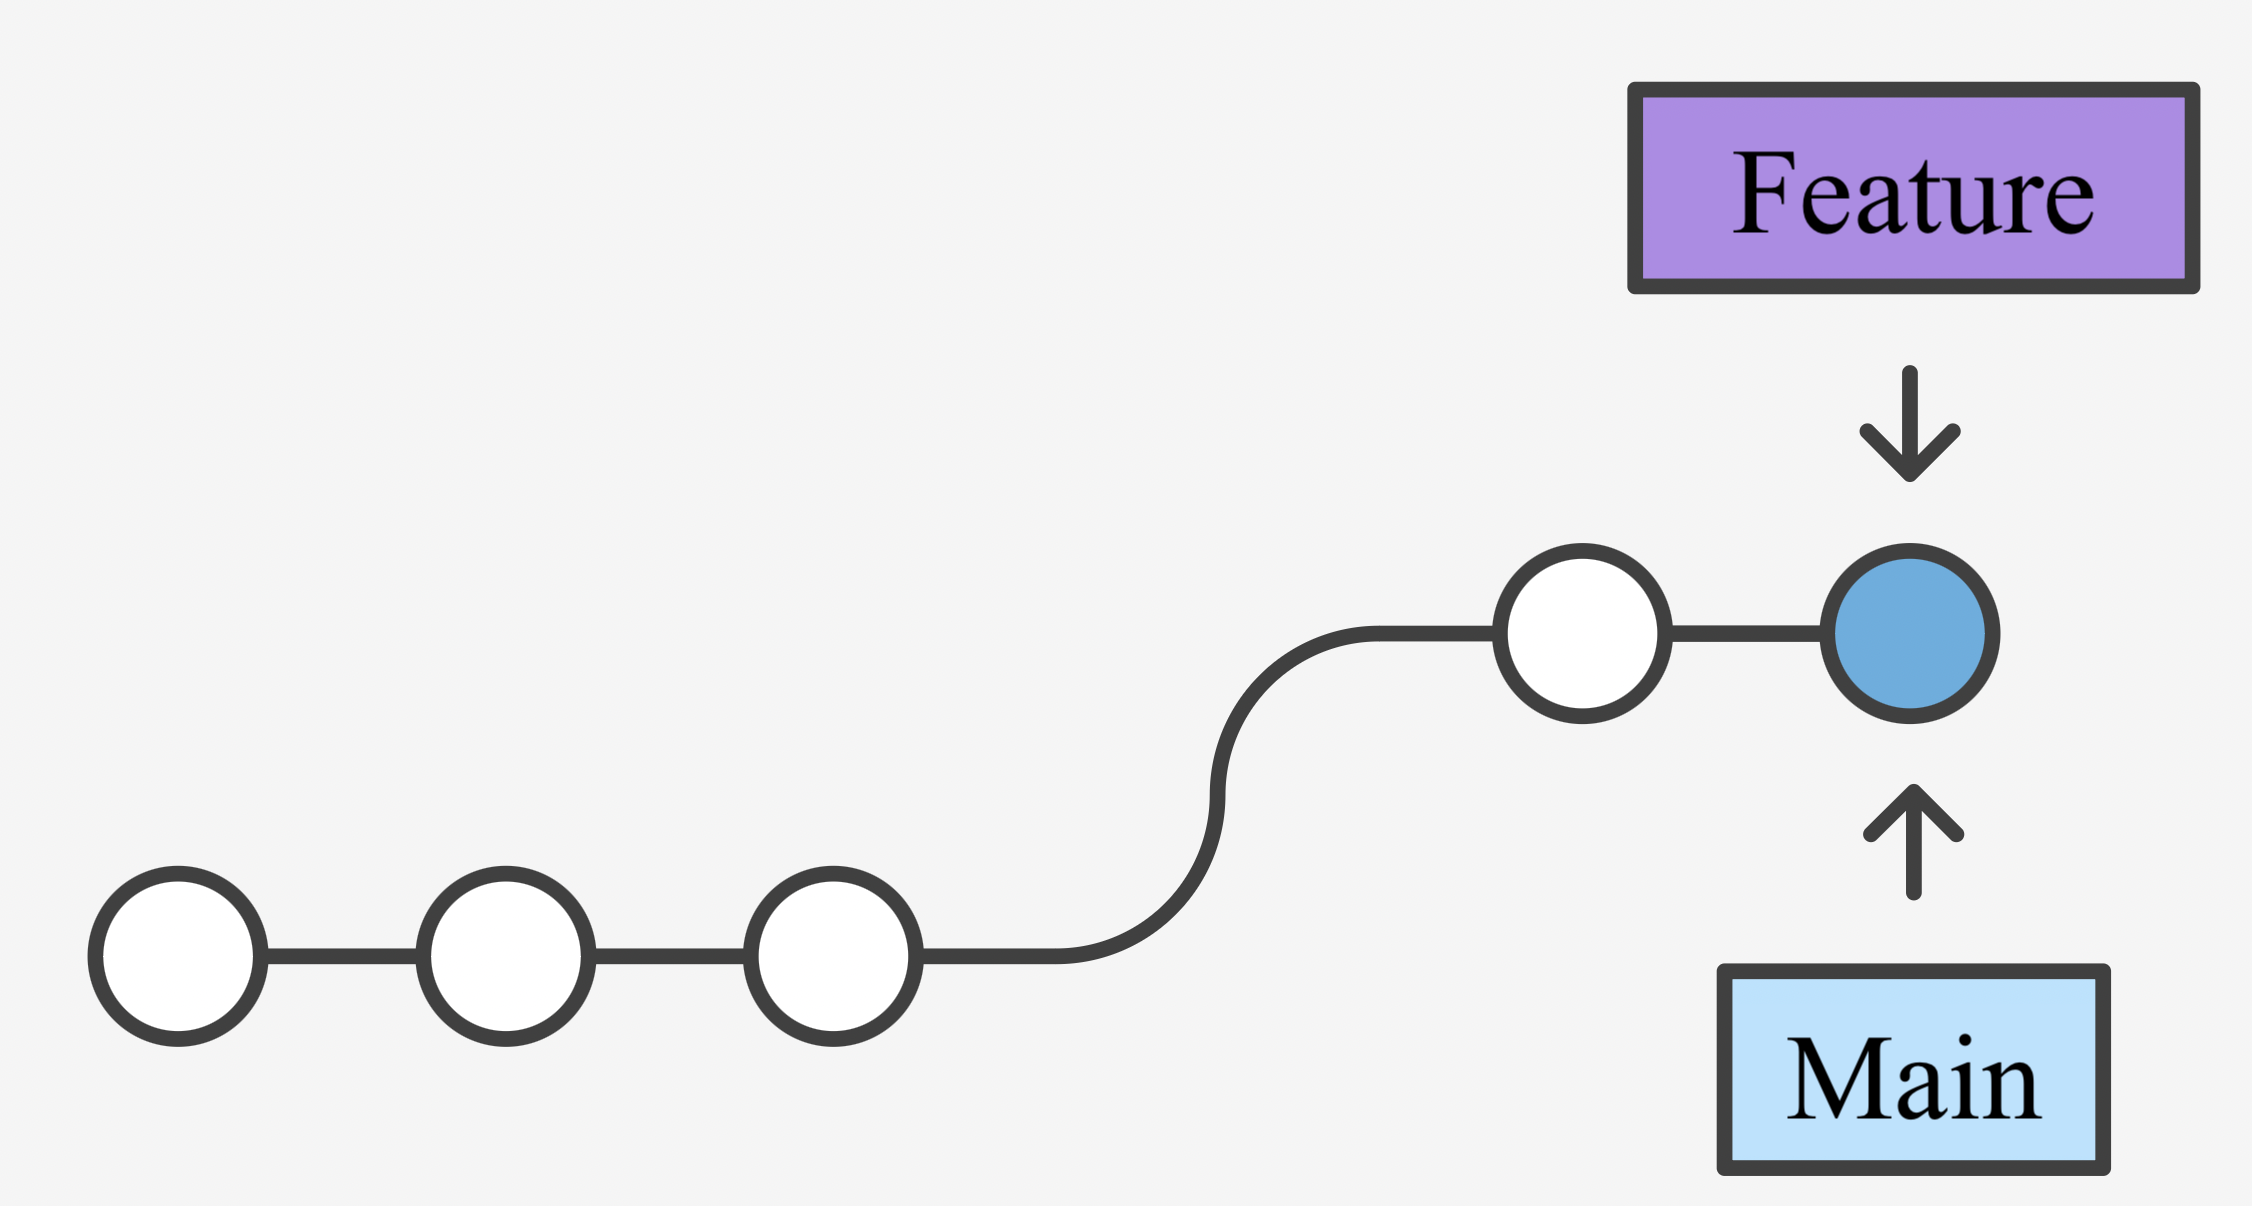
\includegraphics[width=\textwidth]{images/fast_forward_merge_after.png} 
				\captionsetup{justification=centering}
				\captionof{figure}{After fast-forward merge. \href{https://www.atlassian.com/git/tutorials/using-branches/git-merge}{ \faLink{}  Source}}
			\end{minipage}
			% End figure
			\begin{itemize}
				\item A \textcolor{emphasiscolor}{3-way merge} happens when histories between two branches diverge. This can result in a Git conflict. i.e.,
			\end{itemize}
			% Start figure
			\hfill
			\begin{minipage}{0.35\textwidth} 
				\centering
				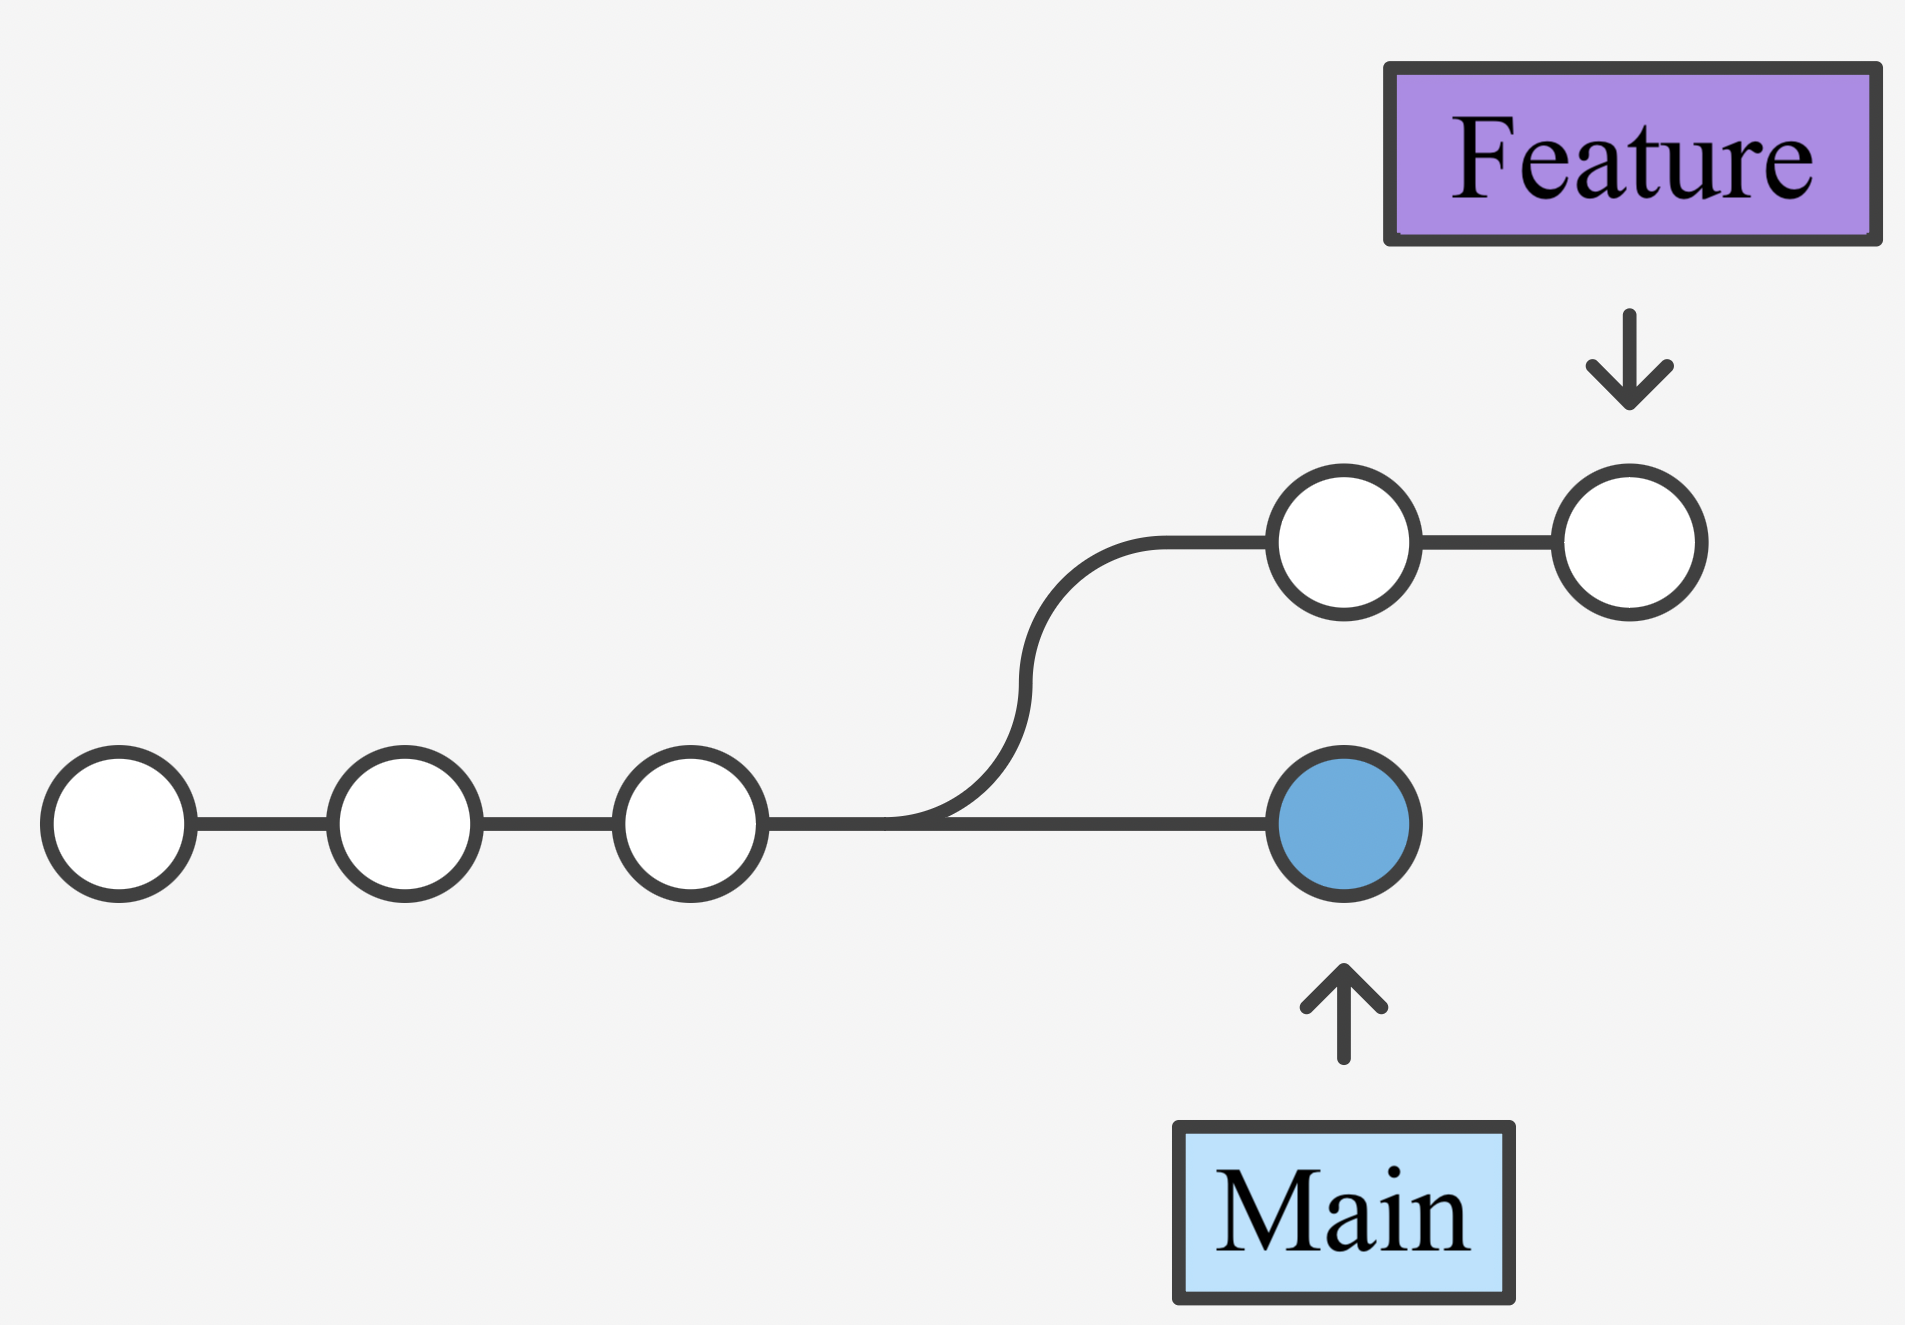
\includegraphics[width=\textwidth]{images/3_way_merge_before.png}
				\captionsetup{justification=centering}
				\captionof{figure}{Before 3-way merge. \href{https://www.atlassian.com/git/tutorials/using-branches/git-merge}{\faLink{} Source}}
			\end{minipage}%
			\hfill
			\begin{minipage}{0.45\textwidth}
				\centering
				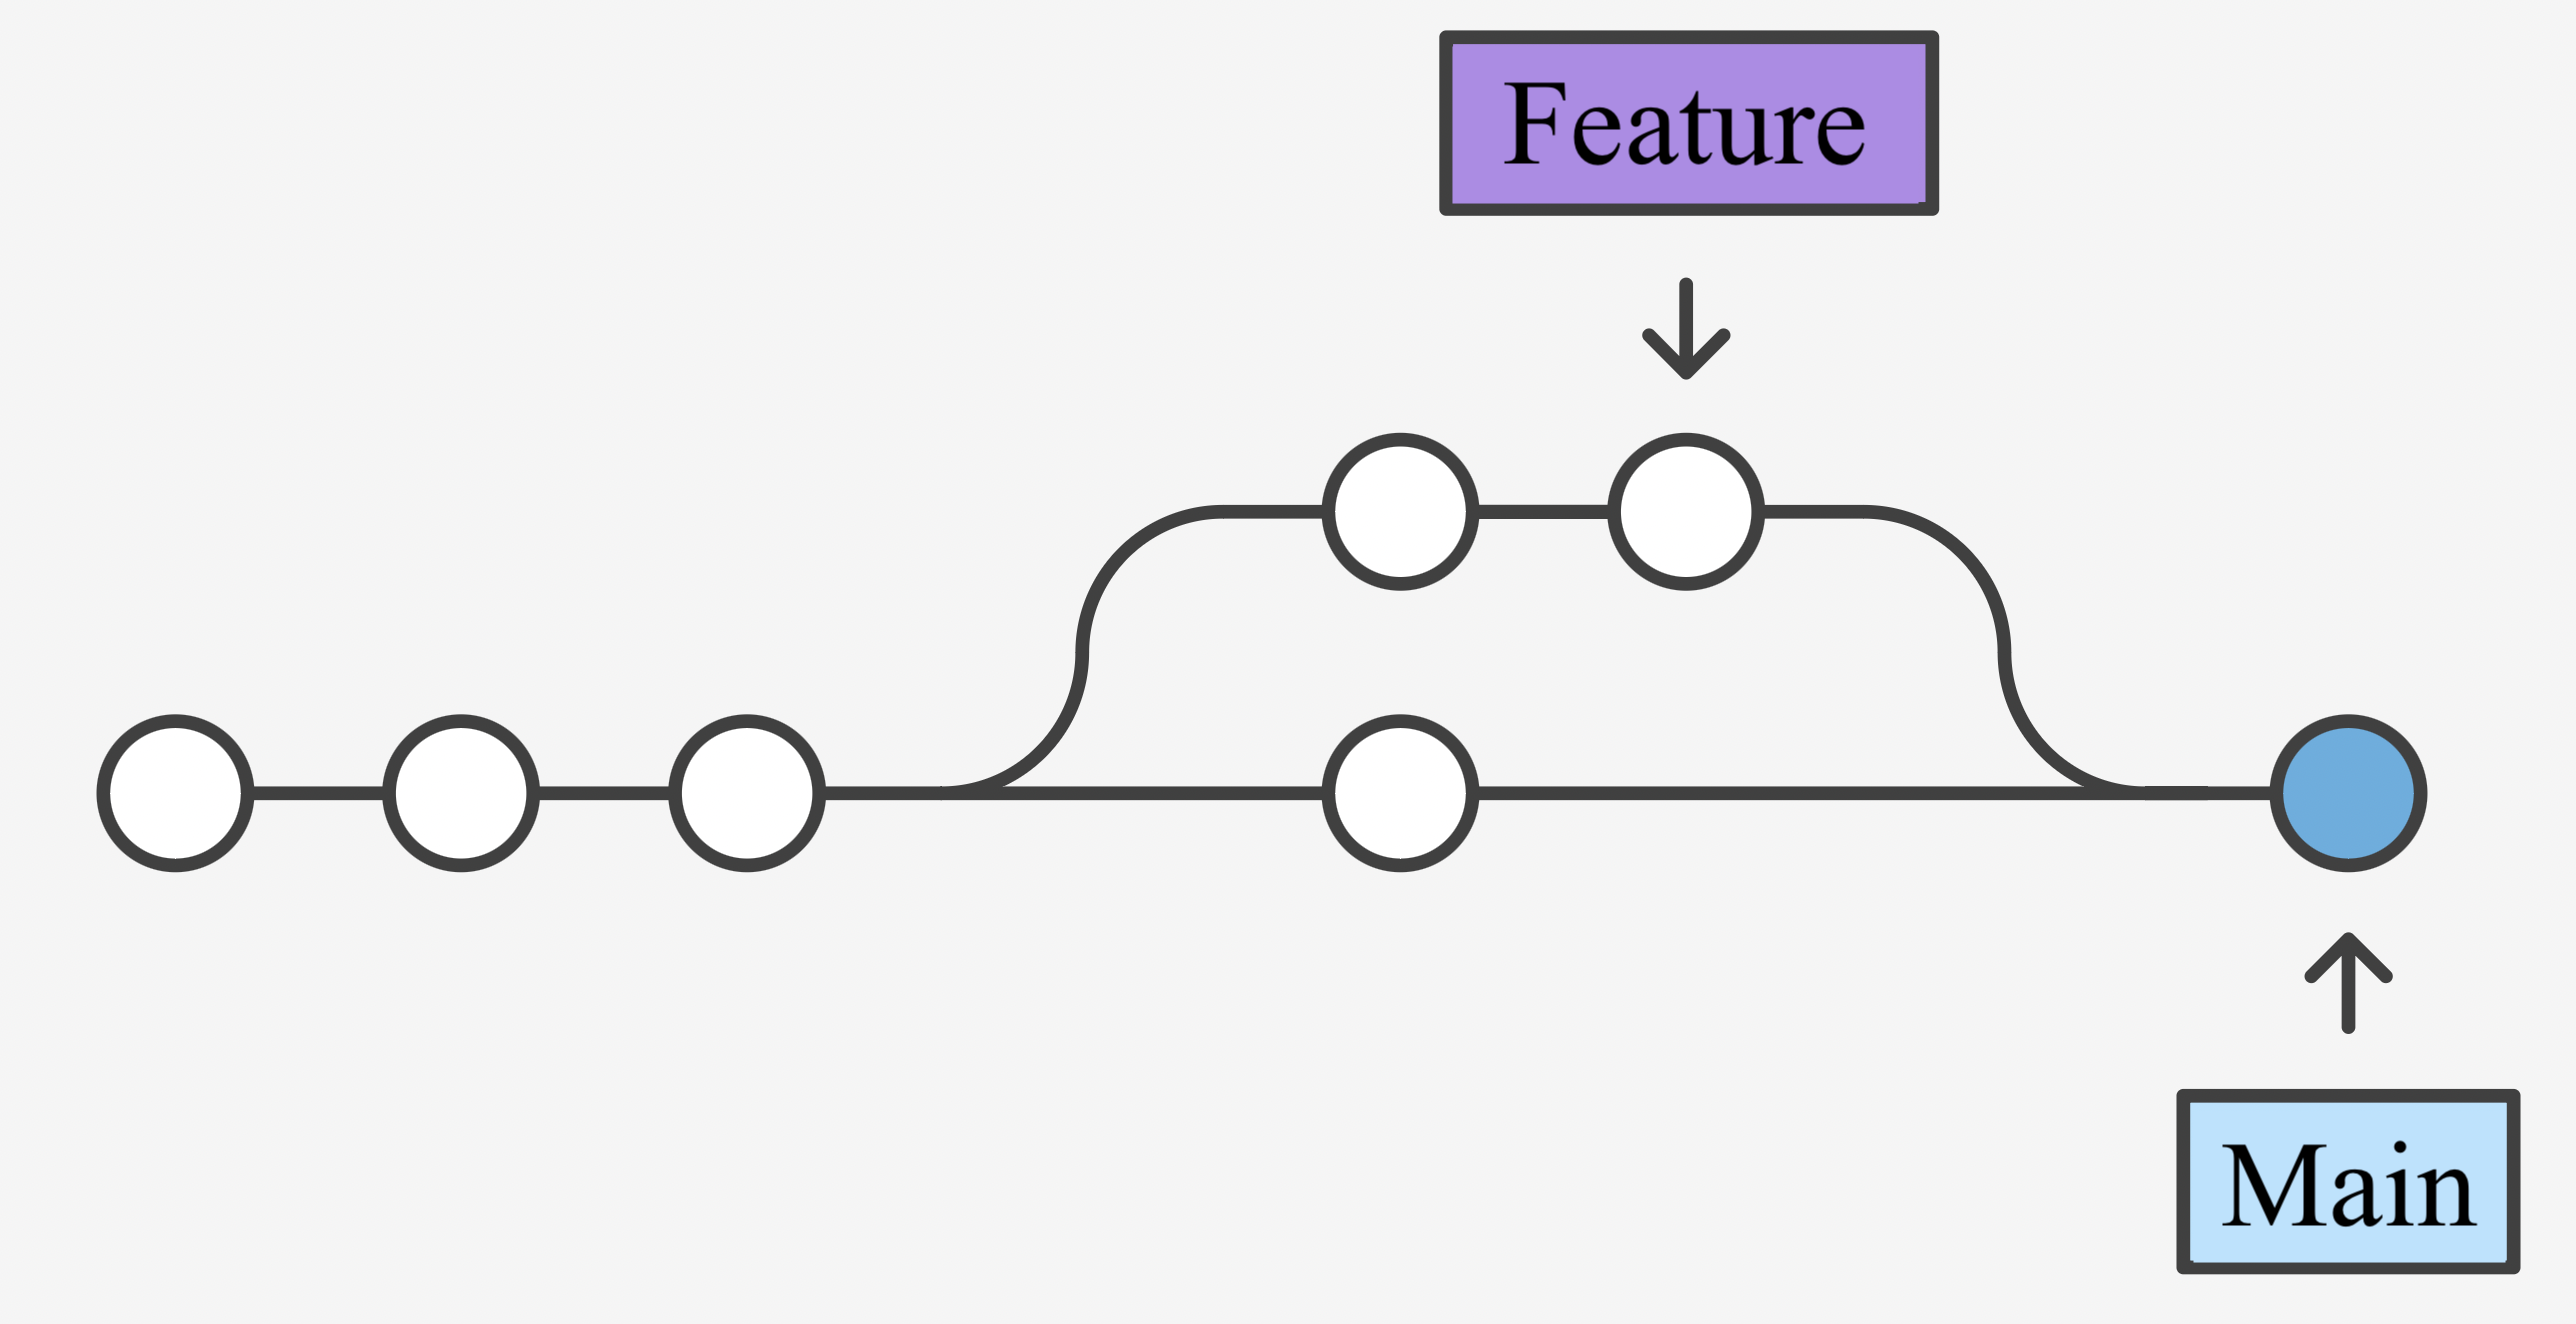
\includegraphics[width=\textwidth]{images/3_way_merge_after.png} 
				\captionsetup{justification=centering}
				\captionof{figure}{After 3-way merge. \href{https://www.atlassian.com/git/tutorials/using-branches/git-merge}{ \faLink{}  Source}}
			\end{minipage}
			% End figure
			
			\vspace{2mm}
			
			Either way, you can \textcolor{emphasiscolor}{squash} multiple commits into one as you merge. This ensures that your commit history size remains manageable. Of course, \href{https://www.geeksforgeeks.org/merge-strategies-in-git/}{less common merge types} do exist for very specific situations. \\
			
		
			\underline{Rebasing}: \textcolor{emphasiscolor}{rewrite the commit history} by "rewinding" the changes from one branch onto another. This means moving commits around.
			\begin{itemize}
				\item \textit{Why?}  This lets you \textcolor{emphasiscolor}{maintain a linear project history} when your feature and master branches start to diverge. It also eliminates the unnecessary merge commits required by merging.
			\end{itemize}
			
		\end{minipage}
	};
	\node[fancytitle, right=10pt, fill=outlinecolor, text=background, draw=outlinecolor, rounded corners] at (box.north west) {Branches};
\end{tikzpicture}



\begin{tikzpicture}
	\node [mybox, fill=boxcolor, draw=outlinecolor] (box){%
		\begin{minipage}{0.3\textwidth}
			\vspace{0.1cm}
			
			\begin{itemize}
				\item \textit{Pull with a rebase.} You can pull changes from \inlinebash{main} into your feature branch as a rebase. This keeps your Git history flat. Use \inlinebash{git pull --rebase origin master}.
			\end{itemize}
			
			The \textcolor{emphasiscolor}{Golden Rule of Rebasing} is do \textcolor{emphasiscolor}{\textbf{not}} rebase on \textcolor{emphasiscolor}{\textbf{public branches}}. 
			\begin{itemize}
				\item \textit{Why?} Branch histories can diverge. This can only be resolved with a merge, which would pollute the commit history. 
				\item \textit{More info.} Check out  \href{https://www.atlassian.com/git/tutorials/merging-vs-rebasing#the-golden-rule-of-rebasing}{this explanation}.
			\end{itemize}
			\smallskip
	
			% Start figure
			\begin{minipage}{\textwidth}
				\centering
				%				\vspace{-2mm}
				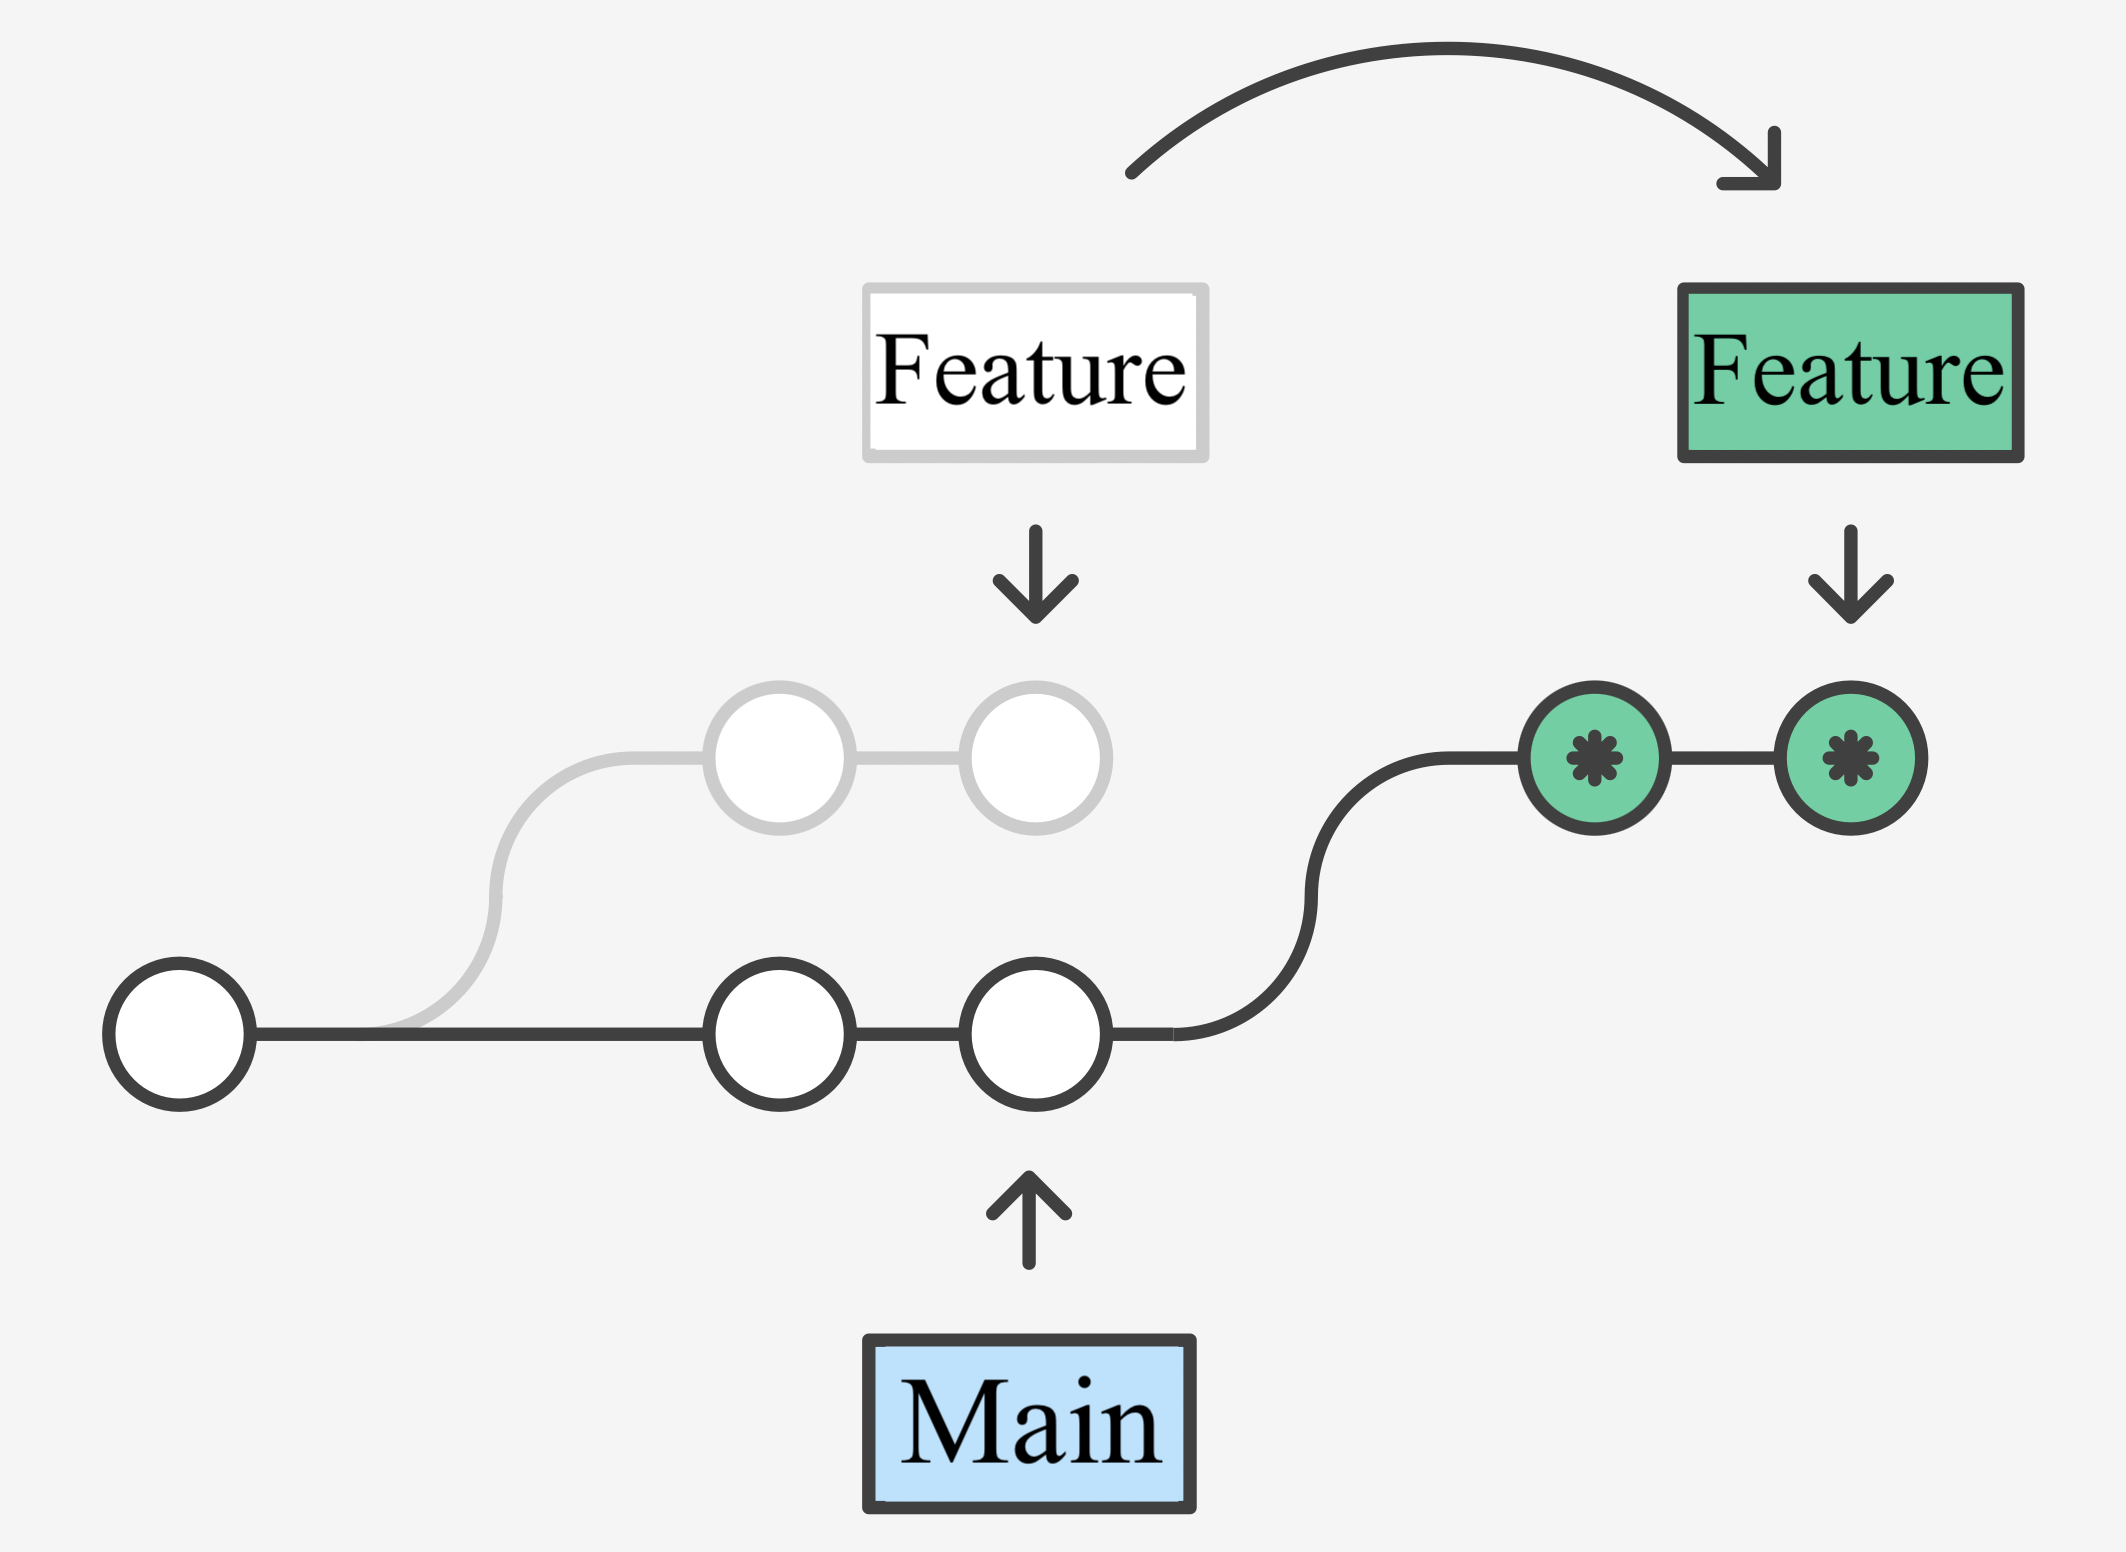
\includegraphics[width=0.5\textwidth]{images/rebase_visualized.png}
				\vspace{-2mm}
				\captionof{figure}{The effects of a \inlinebash{git rebase}. \href{https://www.atlassian.com/git/tutorials/rewriting-history/git-rebase}{ \faLink{}  Source}}
			\end{minipage}
			\vspace{2mm}
		
		\underline{Branching strategies}: the strategy chosen by a software development teams when writing, merging and deploying code. Here are some noteworthy ones:
		\begin{enumerate}
			\item \href{https://nvie.com/posts/a-successful-git-branching-model/}{GitFlow} allows for parallel development to protect the production code. \href{https://www.abtasty.com/blog/git-branching-strategies/#gitflow}{Many variants exist.} It has the following types of branches:
		\end{enumerate}
		\vspace{-2mm}
		\begin{center}
			\textcolor{background}{
				\begin{tabularx}{\textwidth}{>{\columncolor{rowcolor1}}X|>{\columncolor{rowcolor2}}p{6cm}}
					\arrayrulecolor{boxcolor} % Table line color
					\rowcolor{headercolor} % Header row color
					\multicolumn{1}{c|}{\centering \textbf{Branch}} & \multicolumn{1}{c}{\centering \textbf{Description}} \\ % Center the header text
					\hline % Add a horizontal line below the header row
					\rowcolor{rowcolor1} % New Row
					\tablebash{master} & The code that's in production \\
					\rowcolor{rowcolor2} 
					\tablebash{develop} & Where developers merge their features into. Branches off of \tablebash{master}. \\
					\rowcolor{rowcolor1} % New Row
					\tablebash{feature} & One new feature per branch. Branches off of \tablebash{develop}. Merge back once stable. \\
					\rowcolor{rowcolor2} % New Row
					\tablebash{release} & Prepare for a new production release, needs to be merged back into \tablebash{master} and \tablebash{develop}. \\
					\rowcolor{rowcolor1} % New Row
					\tablebash{hotfix} & Fix a bug that has been discovered and must be resolved (usually from production) \\
				\end{tabularx}
			}
		\end{center}
		\vspace{-4mm}
		
		\begin{enumerate}
			\setcounter{enumi}{1} % Set the starting number to 5
			\item In \href{https://www.atlassian.com/continuous-delivery/continuous-integration/trunk-based-development}{trunk-based development}, developers merge small, frequent updates to a core “trunk” or \inlinebash{main} branch. You \textbf{push directly} into \inlinebash{master} and use \inlinebash{release} branches.
			\item \href{https://martinfowler.com/articles/ship-show-ask.html}{Ship / Show / Ask} has three categories for merges:
		\end{enumerate}
		\vspace{-3mm}
		\begin{center}
			\textcolor{background}{
				\begin{tabularx}{\textwidth}{>{\columncolor{rowcolor1}}X|>{\columncolor{rowcolor2}}p{6cm}}
					\arrayrulecolor{boxcolor} % Table line color
					\rowcolor{headercolor} % Header row color
					\multicolumn{1}{c|}{\centering \textbf{Category}} & \multicolumn{1}{c}{\centering \textbf{Description}} \\ % Center the header text
					\hline % Add a horizontal line below the header row
					\rowcolor{rowcolor1} % New Row
					Ship &  Make a change \textbf{directly} into your mainline. Great for updated docs, unremarkable bug fixes; etc. \\
					\rowcolor{rowcolor2} 
					\tablebash{Show} & Open a Pull Request with your change but merge without waiting for anyone. \\
					\rowcolor{rowcolor1} 
					\tablebash{Ask} & Open a Pull Request and wait for approval before merging  \\
				\end{tabularx}
			}
		\end{center}
		
		\end{minipage}
	};
	\node[fancytitle, right=10pt, fill=outlinecolor, text=background, draw=outlinecolor, rounded corners] at (box.north west) {Branches (2)};
\end{tikzpicture}